\message{ !name(article.tex)}%%%%%%%%%%%%%%%%%%%%%%%%%%%%%%%%%%%
%This is the LaTeX ARTICLE template for RSC journals
%Copyright The Royal Society of Chemistry 2016
%%%%%%%%%%%%%%%%%%%%%%%%%%%%%%%%%%%

\documentclass[twoside,twocolumn,9pt]{article}
\usepackage{extsizes}
\usepackage[super,sort&compress,comma]{natbib} 
\usepackage[version=3]{mhchem}
\usepackage[left=1.5cm, right=1.5cm, top=1.785cm, bottom=2.0cm]{geometry}
\usepackage{balance}
\usepackage{mathptmx}
\usepackage{sectsty}
\usepackage{graphicx}
\usepackage{subcaption}
\usepackage{lastpage}
\usepackage[format=plain,justification=justified,singlelinecheck=false,font={stretch=1.125,small,sf},labelfont=bf,labelsep=space]{caption}
\usepackage{float}
\usepackage{fancyhdr}
\usepackage{fnpos}
\usepackage[english]{babel}
\addto{\captionsenglish}{%
  \renewcommand{\refname}{Notes and references}
}
\usepackage{array}
\usepackage{droidsans}
\usepackage{charter}
\usepackage[T1]{fontenc}
\usepackage[usenames,dvipsnames]{xcolor}
\usepackage{setspace}
\usepackage[compact]{titlesec}
\usepackage{hyperref}
\usepackage{todonotes}
\usepackage{siunitx}
%%%Please don't disable any packages in the preamble, as this may cause the template to display incorrectly.%%%


\usepackage{epstopdf}%This line makes .eps figures into .pdf - please comment out if not required.

\definecolor{cream}{RGB}{222,217,201}

\graphicspath{{Figures/}}

\begin{document}

\message{ !name(article.tex) !offset(202) }
t alterations, excepting sodium sulphate which was oven dried 24 hours
before use.
Deuterated 1-decanol (DeOH-$\alpha$-d$_2$) was synthesized by reducing ethyl
decanoate (\ce{C12H24O2}) with lithium aluminum deuteride (\ce{LiAlD4}) and
purified by vacuum fractional distillation.\\

\begin{figure}[h]
\centering
  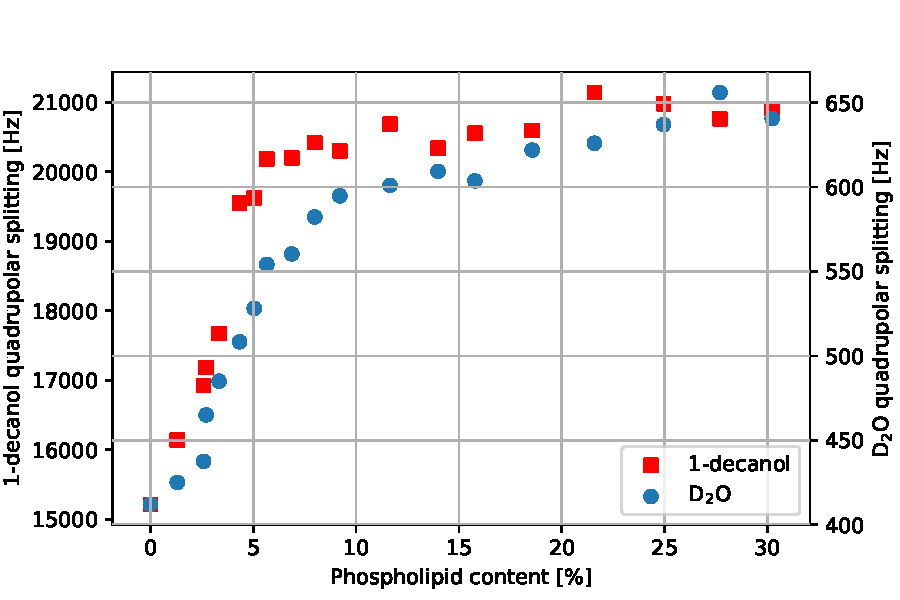
\includegraphics[width=\columnwidth]{splitting_v_phospholipid}
  \caption{Quadrupolar splittings of 1-decanol-$\alpha$-$d_2$ and \ce{D2O} in
    $^2$H-RMN as a function of the phospholipid content in the mimetic.}
  \label{fig:1st_max}
\end{figure}

In order to achieve a membrane mimetic that behaves as similar as possible to
the actual cellular membrane, it is necessary to maximize its phospholipid
concentration. This is important considering that multiple researchers have
concluded that there are specific interactions between the phosphate from the
multiple phospholipids and certain amino-acids that modify the membrane
permeability where this interaction occurs\cite{Aliaga2011,Hristova2011}.\\
Also, the membrane mimetic must orient itself in presence of an external
magnetic field. This is so the deuterated probes in the mimetic can produce a
\textit{quadrupole splitting} in its $^2$H-RMN spectrum, which will be used to
assess the mobility, location and orientation of each deuterium labeled component.\\
Both these requirements were fulfilled by employing the membrane mimetic
developed by Bahamondes \textit{et al}\cite{Bahamonde-Padilla2013} as starting
point, then introducing and maximizing the concentration of phospholipid onto
this composition. The maximization was performed in two steps. In a first step,
a batch of membrane mimetics was prepared, each one with an increasing amount of
phospholipid from 0\% up to 30\% (see figure \ref{fig:1st_max}), $^2$H-RMN
spectra and polarized light microscopy pictures were taken to each prepared
membrane mimetic. From these, the composition with 22\% of phospholipid was
chosen to continue with the next maximization step, as this was the composition
with highest phospholipid content that retained a $^2$H-NMR spectrum
characteristic of a nematic phase (see figure \ref{fig:22v23}).\\

\begin{figure}[h]
  \centering
  \begin{subfigure}{0.45\columnwidth}
    \includegraphics[width=\linewidth]{schlieren_1max}
    \caption{4\% Phospholipid}
    \label{fig:schlieren}
  \end{subfigure}
  \begin{subfigure}{0.45\columnwidth}
    \includegraphics[width=\linewidth]{oily_17percent}
    \caption{17\% Phospholipid}
    \label{fig:oily}
  \end{subfigure}
  \caption{Polarized light microscopy pictures of membrane mimetics at different
  phospholipid concentration. Both pictures taken at 100x zoom.}
  \label{fig:plm}
\end{figure}

During this step of maximization, we noticed a phase transition upon reaching
6\%-10\%, this phase transition was also evidenced by polarized light microscopy
(see figure \ref{fig:plm}) where a transition from a \textit{Schlieren} pattern
(fig. \ref{fig:schlieren}) to an \textit{oily streak} pattern (fig.
\ref{fig:oily}) was observed. While both patterns are characteristic of
lyotropic nematic phases, further experiments are required to assess the exact
structure of each phase.

\begin{figure}[h]
\centering
  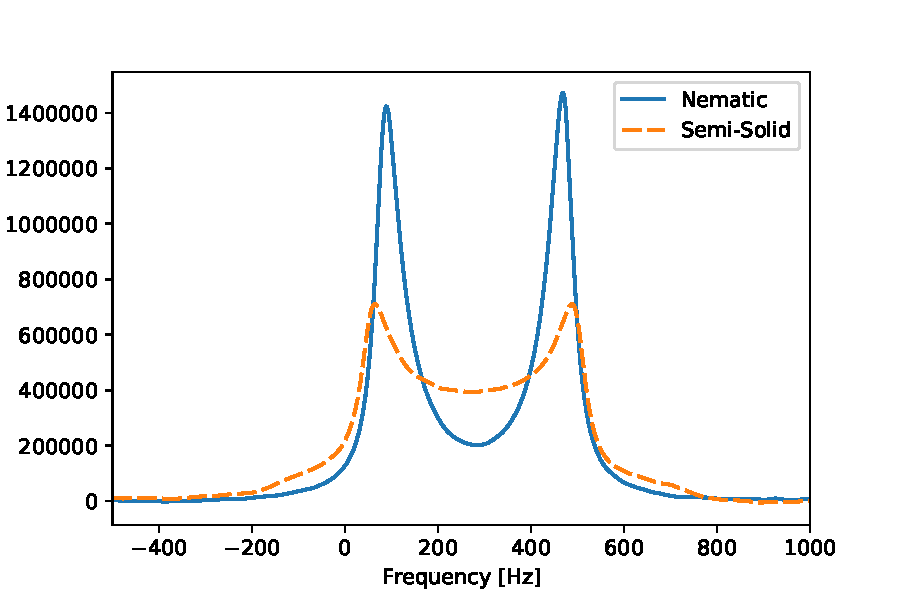
\includegraphics[width=\columnwidth]{nematic_v_semisolid}
  \caption{Comparison between $^2$H-NMR spectra from HDO in nematic and
    semi-solid phases}
  \label{fig:22v23}
\end{figure}

The second maximization step was performed by reducing the amount of SDS used to
prepare each mimetic and subsequently adding phospholipid until a nematic phase
was no longer obtained. The results from the membrane mimetic candidates
prepared in this step are summarized in figure \ref{fig:phase_diag}. From these
preparations, again, the composition with the highest phospholipid content that
retained a nematic phase was chosen for further experimentation. The exact
composition of the membrane mimetic is detailed in table \ref{tab:mimetic_composition}

\begin{figure}[h]
\centering
  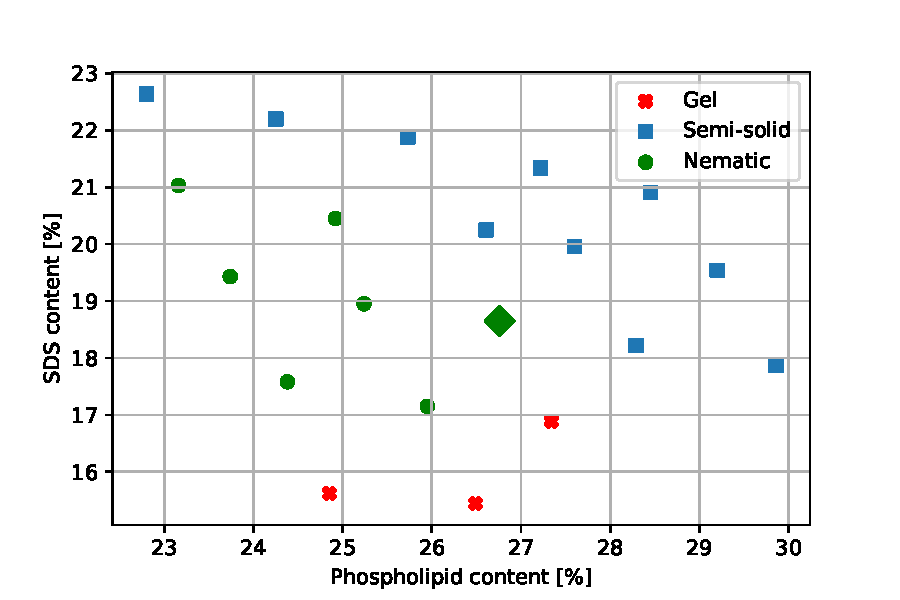
\includegraphics[width=\columnwidth]{phase_diag}
  \caption{Partial phase diagram of the membrane mimetic when varying SDS and
    phospholipid content. The selected composition is marked as a green diamond.}
  \label{fig:phase_diag}
\end{figure}

\begin{table}[h]
\small
  \caption{\ }
  \label{tab:mimetic_composition}
  \begin{tabular*}{0.48\textwidth}{@{\extracolsep{\fill}}ll}
    \hline
    Compound & Content [$\tfrac{w}{w}\%$] \\
    \hline
    Sodium dodecyl sulphate &  18.65\% \\
    Sodium sulphate & 1.55\%  \\
    1-decanol & 3.92\%  \\
    Phospholipid mixture & 26.76\%  \\
    Water & 49.12\% \\
    \hline
  \end{tabular*}
\end{table}

\section{Calibration of a computational model}
\label{sec:calib}

In order to obtain significant information from a molecular dynamic simulation,
it has to be calibrated to reproduce known experimental results. \par As a first
step, three force-fields with different partial charge distributions were
tested. These force-fields were chosen due to their ability to reproduce
structures of SDS aggregates\cite{Tang2014}.\par
The tested force-fields were:
\begin{itemize}
\item CHARMM36\cite{Vanommeslaeghe2009}
\item Berger\cite{Berger1997} with partial charge distribution according to Merz-Kollman
  method\cite{Besler1990}
\item Berger with partial charge distribution according to Gromos53A6\cite{Oostenbrink2004}
  parameters.
\item Gromos53A6 with partial charge distribution according to Merz-Kollman
  method. And
\item Gromos53A6 with partial charge distribution according to its own parameters.
\end{itemize}

All simulations were performed using the GROMACS-2016\cite{Abraham2015} software
bundle. A cutoff scheme was used for non-bonding interactions according to each
force-field recommendation values. Temperature control was achieved with a
modified Berendsen thermostat\cite{Bussi2007}, while pressure was equilibrated
with a semi-isotropic Berendsen barostat\cite{Berendsen1984}. Both temperature
and
pressure were adjusted to \SI{310}{K} and \SI{1}{bar} respectively.\\
Before each production simulation, a short equilibration run was performed for a
duration of \SI{1}{ns} with an integration time-step of \SI{1}{fs}. Afterwards,
each production run was calculated to a duration of \SI{40}{ns} with an
integration time-step of \SI{2}{fs}. TIP3P water model was employed on the
simulation with CHARMM36 force-field, while SPC/E was employed on simulations
with Berger and Gromos53A6 force-fields. The same initial configuration was
employed to test each force-field, and it was generated using the software
Packmol\cite{Martinez2009} arranging a bilayer with composition in the same
proportion as the membrane mimetic in table \ref{tab:mimetic_composition} to a
total of 9613 molecules. The phospholipid mixture was simulated as a mixture of
39\% PLPC, 26\% DLPC, 24\% DLPE and 11\% DOPE. These proportions were chosen in
accordance with the composition of the phospholipid mixture employed.\\

From each resulting simulation run, deuterium order parameters ($S_{CD}$) were calculated
for the SDS aliphatic chain, which were used to calculate a predicted qudrupolar
splitting employing equation \ref{eq:splitting} which depends on a coupling
constant ($e^2qQ/h$) and the angle ($\theta$) between the normal to the bilayer and the
applied magnetic field.

\begin{equation}
  \label{eq:splitting}
  \Delta\nu = \frac{3}{4} \frac{e^2qQ}{h}(3\cos^2\theta - 1) S_{CD}
\end{equation}

These predicted qudrupolar splittings were compared with experimental results,
as shown in figure \ref{fig:calibration}, concluding that employing the
Gromos53A6 force-field yields the results that are closer to experimental ones
(see figure \ref{fig:reference}), obtaining a good correlation on the carbons
near to the interface and diverging towards the interior of the bilayer.

\begin{figure}[h]
  \centering
  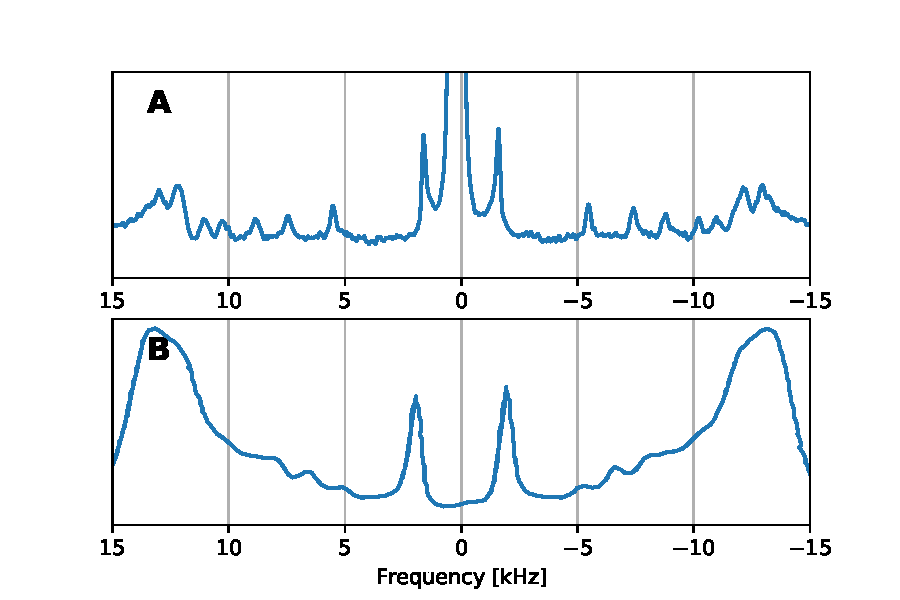
\includegraphics[width=\columnwidth]{nmr_reference}
  \caption{$^2$H-NMR spectrum of membrane mimetic enriched with SDS-d$_{25}$.
    Central peak (not shown completely) belongs to \ce{HDO} present in the
    sample, while the rest of the signals are split SDS-d$_{25}$ signals which
    were used as reference to calibrate a computational model.}
  \label{fig:reference}
\end{figure}
\begin{figure}[h]
\centering
  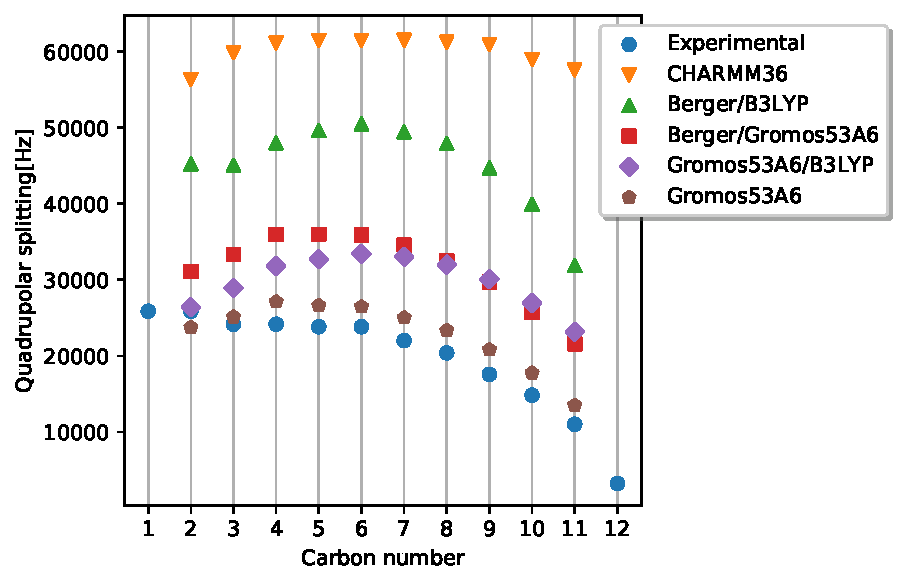
\includegraphics[width=\columnwidth]{calibration}
  \caption{Quadrupolar splittings of SDS-d$_{25}$ from a $^2$H-NMR. Comparison
    between experimental results and predicted by molecular dynamics employing
    different force-fields}
  \label{fig:calibration}
\end{figure}

Further improvement was done to the fitting of predicted results by employing
two thermostats in the simulation, one governing the bulk solution with a
reference temperature of \SI{310}{K} and another governing the bilayer
components with a reference temperature of \SI{320}{K}. The reasoning behind
this decision was based on the expectation that the increased velocity on the
bilayer components would have a further effect on the mobility towards the
center on the bilayer rather than in the interface, where Coulombic interactions
are stronger and have a restraining effect on the mobility of the bilayer. After
this adjustment, the simulation results in predicted quadrupolar splittings in
very good agreement with the experimental ones, as shown in figure
\ref{fig:2nd_calibration}.

\begin{figure}[h]
\centering
  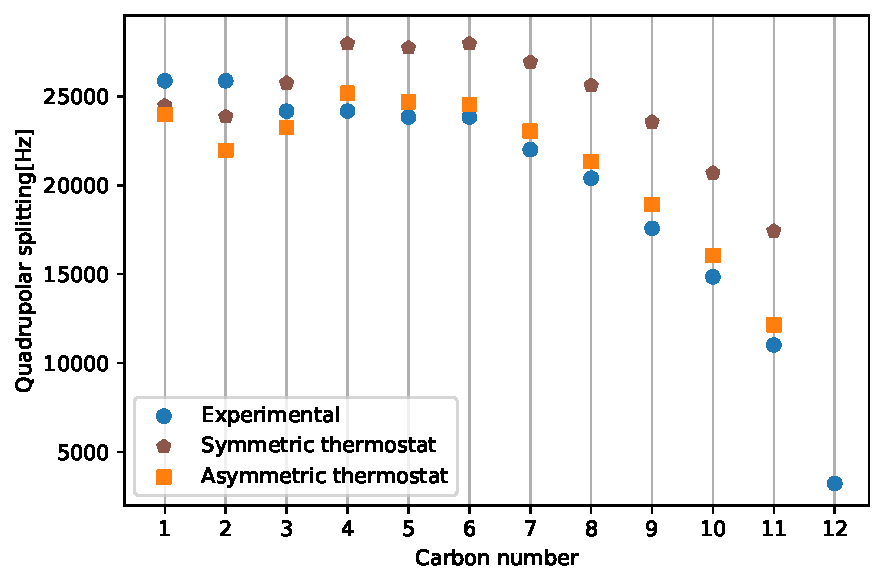
\includegraphics[width=\columnwidth]{calibration2}
  \caption{Quadrupolar splittings of SDS-d$_{25}$ from a $^2$H-NMR. Comparison
    between experimental results and predicted by molecular dynamics with
    symmetric and asymmetric thermostat}
  \label{fig:2nd_calibration}
\end{figure}

\section{Membrane mimetic validation}
\label{sec:validation}

In order to corroborate that the composition achieved (table
\ref{tab:mimetic_composition}) behaves as a membrane mimetic, we tested the
permeation properties of two drugs: Benzocaine, that is known to be able to passively
cross the cellular membrane; and Levodopa, which is known to be able to cross the
cellular membrane via active mechanisms, therefore it should not be able to
permeate a membrane mimetic without specific receptors.

\subsection{Benzocaine control}
\label{sec:benzo}

\begin{figure}[htb]
  \centering
  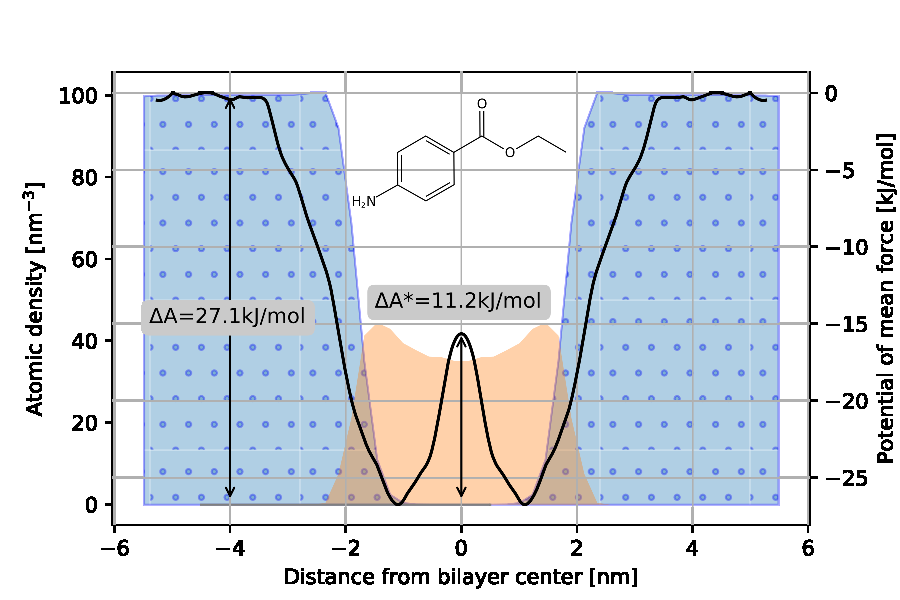
\includegraphics[width=\columnwidth]{benzo_profile_density}
  \caption{Mean force potential profile for the process of Benzocaine
    translocating through a membrane mimetic. The blue dotted area represents
    the water particle density, while the smooth orange area represents the
    lipid particle density in the simulation.}
  \label{fig:benzocaine_profile}
\end{figure}
Employing the calibrated model stated before, a potential of mean force (PMF)
profile was calculated for the process of Benzocaine permeating the membrane
(figure \ref{fig:benzocaine_profile}) employing the Umbrella
Sampling/WHAM\cite{Kumar1992} method. From this PMF profile it can be
deduced that Benzocaine goes through three steps in order to complete its
translocation: First, it integrates spontaneously with the outer leaflet of the
bilayer, without mayor interactions with the Stern layer. Secondly, Benzocaine
``flip-flops'' to the inner leaflet of the bilayer with a small activation
energy (\SI{11.2}{\kilo\joule}). And third and finally, it escapes the bilayer
into the
bulk at a minor energetic cost (\SI{27.1}{kJ}), showing that Benzocaine
permeation through the membrane mimetic is indeed possible.\\
\begin{figure}[htb]
  \centering
  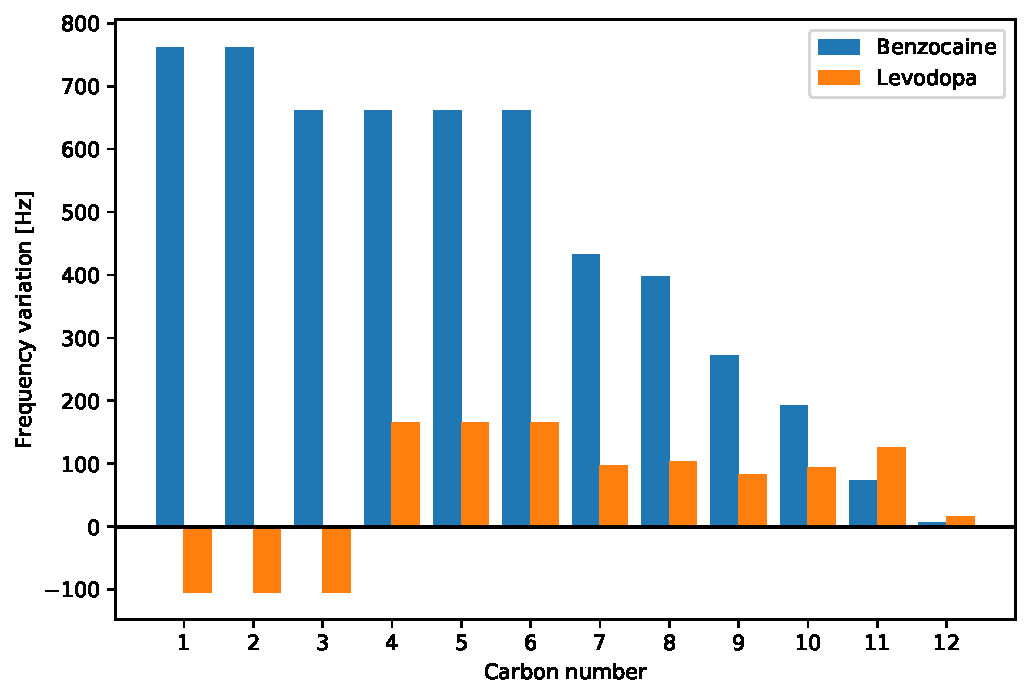
\includegraphics[width=\columnwidth]{sds_variation}
  \caption{Variation on quadrupolar splittings in $^2$H-NMR upon adding
    Benzocaine or Levodopa to a membrane mimetic sample enriched with
    SDS-d$_{25}$.}
  \label{fig:sds_benzocaine}
\end{figure}
$^2$H-NMR spectum was taken from a membrane mimetic sample with \SI{8}{mg}
Benzocaine added per gram of mimetic enriched with SDS-d$_{25}$, and compared to
a spectrum of the same mimetic without the anesthetic (figure
\ref{fig:sds_benzocaine}). From this result, it can be seen that the presence of
Benzocaine alters the quadrupolar splittings of the SDS aliphatic chain from the
first up to the sixth carbon, implying that Benzocaine is mostly residing in
this area, this is concordant with the results of the PMF profile (figure
\ref{fig:benzocaine_profile}), which shows that the most stable position for the
Benzocaine to be in, is indeed inside the bilayer and closer to the interface.



\subsection{Levodopa control}
\label{sec:ldopa}

Employing the same method as in Benzocaine, a PMF profile was calculated for the
process of Levodopa permeating the membrane mimetic (figure
\ref{fig:levodopa_profile}). This profile shows that the position of lowest
energy for Levodopa to be in, is outside the bilayer, alongside the Stern layer;
it also shows that in order to permeate the bilayer, Levodopa requires a rather
large activation energy (\SI{102.4}{\kilo\joule\per\mol}) in order to translocate
through the membrane, showing that a passive permeation of Levodopa through the
membrane mimetic is actually not possible.

\begin{figure}[htb]
  \centering
  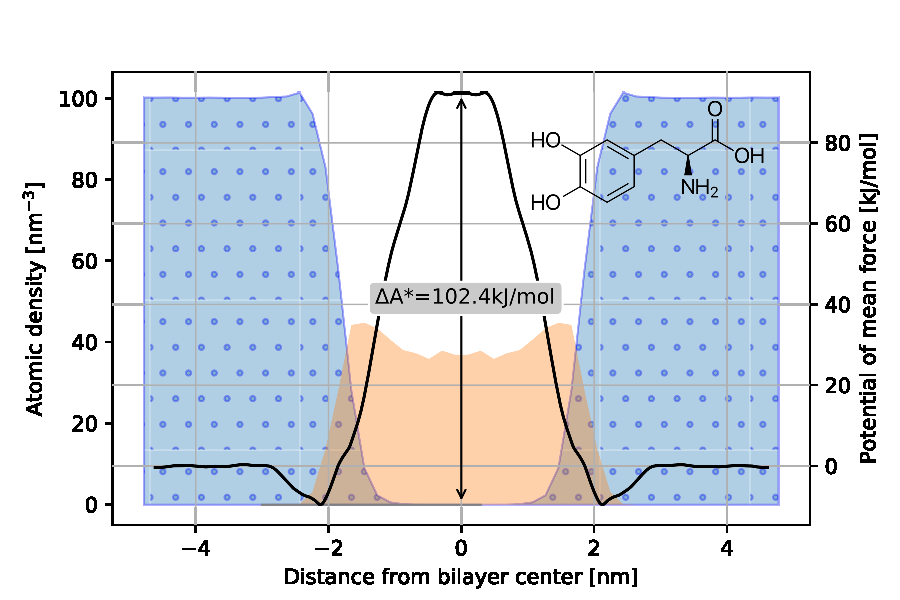
\includegraphics[width=\columnwidth]{ldopa_profile_density}    
  \caption{Mean force potential profile for the process of Levodopa
    translocating through a membrane mimetic. The blue dotted area represents
    the water particle density, while the smooth orange area represents the
    lipid particle density in the simulation.}
  \label{fig:levodopa_profile}
\end{figure}

This previous result is supported by $^2$H-NMR spectra. When studying the
effects of adding \SI{7}{mg} of Levodopa per gram of membrane mimetic enriched
with SDS-d$_{25}$ the effects are minor to negligible (see figure \ref{fig:sds_benzocaine}),
implying that the Levodopa molecules are unable to enter the bilayer to alter
its mobility.

\section{Conclusions}
The high phospholipid content present in this membrane mimetic makes it better
at reproducing interactions between proteins (or peptides) and the bilayer,
considering that multiple researchers\cite{Aliaga2011,Hristova2011} have found
that there is an specific interaction between arginine and the phosphate from
each phospholipid
that modify the properties of the membrane where this interaction occurs.\\
Also, the ability to orient itself in an external magnetic field and its sodium
dodecyl sulphate content, which is relatively inexpensive in deuterated form,
makes this membrane mimetic ideal for studies of mobility and orientation
employing $^2$H-NMR.\\
Furthermore, we present a calibrated simulation model employing molecular
dynamics, which as shown with the PMF profiles of Benzocaine and Levodopa, it
allows to obtain information about the translocating process that is usually
unfeasible to obtain via experimental means.\\
And finally, having proven that Benzocaine, a local anesthetic that permeates
the cellular membrane, is able to translocate through the membrane mimetic
proposed in this article; and that Levodopa, an amino-acid that cannot permeate
passively the cellular membrane, is unable to do so thr
\message{ !name(article.tex) !offset(229) }

\end{document}
